\title[P\&S 2026/2027]{Probability \& Statistics (Premaster MTPS)}
\subtitle[College 3]{College 3: schatten en toetsen}  
\author{Dr. ir. D.A.M.P. Blom}
\institute[NLDA]{Nederlandse Defensie Academie}
\date{6 november 2026}

\begin{document}

    \AtBeginSection[]{
        \frame<beamer>{
            \frametitle{Inhoud}

            \tableofcontents[currentsection, currentsubsection]
        }
    }

    \begin{frame}
        \maketitle
        % \begin{center}
        %     \includegraphics[width=3cm]{1_marine}
        %     \includegraphics[width=3cm]{1_luchtmacht}
        %     \includegraphics[width=3cm]{1_landmacht}
        % \end{center}
    \end{frame}


    %------------------------------------------------%	

    \begin{frame}{Agenda}
        Vandaag van 9.20 tot 16.40 uur
        \vfill
        {\small
        \begin{itemize}
            \item 9.20 - 10.00 uur: recap vorige les en lineariteit van de verwachtingswaarde
            \item 10.15 - 11.00 uur: introductie in schattingsmethoden.
            \item 11.15 - 12.00 uur: zuivere schatters en het vergelijken van varianties
            \item 12.45 - 13.30 uur: betrouwbaarheidsintervallen voor $\mu$ ($\sigma$ bekend)
            \item 13.45 - 14.30 uur: betrouwbaarheidsintervallen voor $\mu$ ($\sigma$ onbekend)
            \item 14.45 - 15.30 uur: hypothesetoetsen deel 1 
            \item 15.45 - 16.30 uur: hypothesetoetsen deel 2
        \end{itemize}
        }
        \vfill
        \textbf{Dit komt ruwweg overeen met de stof van learning tasks 11 t/m 15.}
    \end{frame}

%==================================================================
\section{Recap vorige les}
%==================================================================

    \begin{frame}\frametitle{Recap: kansvariabelen}
        {\scriptsize
            \begin{center}
                \begin{tabular}{m{0.45\textwidth}m{0.45\textwidth}}
                    \toprule
                        \textbf{Discrete kansvariabele} & \textbf{Continue kansvariabele}\\
                    \midrule
                        \uncover<+->{$S$ bestaat uit losse, afzonderlijke waarden & $S$ is een spectrum van waarden} \\ \midrule
                        \uncover<+->{kansmassafunctie $f(x) = P(X = x)$: \begin{itemize} \item $f(x) \geq 0$ voor iedere uitkomst $x$ 
                            \item $\sum_{x \in S} f(x) = 1$ \end{itemize}
                            & Kansdichtheidsfunctie $f(x)$: \begin{itemize} \item $f(x) \geq 0$ voor iedere uitkomst $x$
                            \item $\int_{x \in S} f(x) \dx = 1$ \end{itemize}
                            } \\ \midrule
                        \uncover<+->{CDF $F(x) = P(X \leq x) = \sum_{y \leq x} f(y)$
                        \begin{itemize} \item $F$ is monotoon niet-dalend
                                        \item $\lim_{x \to -\infty} F(x) = 0$ en $\lim_{x \to \infty} F(x) = 1$
                                    \end{itemize}
                                    & CDF $F(x) = P(X \leq x) = \int_{-\infty}^x f(y) \dy$
                        \begin{itemize}
                            \item $F$ is monotoon niet-dalend
                            \item $\lim_{x\to-\infty} F(x) = 0$ en $\lim_{x \to \infty} F(x) = 1$
                        \end{itemize}} \\ \midrule
                        \uncover<+->{$E(X) = \sum_{x \in S} x \cdot f(x)$ & $E(X) = \int_{x \in S} x \cdot f(x) \dx$} \\ \midrule
                        \uncover<+->{$\Var{X} = \sum_{x \in S} \left(x - E(X)\right)^2 \cdot f(x)$ & $\Var{X} = \int_{x \in S} \left(x - E(X)\right)^2 \cdot f(x) \dx$} \\ \midrule
                        \uncover<+->{$\sigma(X) = \sqrt{\Var{X}}$ & $\sigma(X) = \sqrt{\Var{X}}$} \\                 
                    \bottomrule
                \end{tabular}   
            \end{center}
        }
        \vfill\pause
        Veelgebruikte verdelingen: normaal $N(\mu, \sigma)$, binomiaal, Poisson.
    \end{frame}

    \begin{frame}\frametitle{Berekeningen met de grafische rekenmachine}
        \only<+>{
            Met \enquote{normalcdf} (2nd-DISTR-2) bereken je de kansen $P(a \leq X \leq b)$ voor gegeven grenswaarden $a$ en $b$ voor een normaal verdeelde kansvariabele $X \sim N(\mu,\sigma)$.
            \begin{center}
                \includegraphics[width=0.9\textwidth]{3_voorbeeld_normalcdf.png}
                \vfill
                \textbf{Syntax:} $\normalcdf(\lb=90, \ub=115, \mu=100, \sigma=15)$
            \end{center}
        }   
        \only<+>{
            Met \enquote{invnorm} (2nd-DISTR-3) bereken je de grenswaarde(n) waarvoor een kans $p$ links / rechts ligt (percentielen).
            \begin{center}
                \begin{tabular}{*{2}{c}}
                    \textbf{Tail$=$LEFT} & \textbf{Tail$=$RIGHT} \\
                    \includegraphics[width=0.45\textwidth]{3_voorbeeld_invnorm_LEFT.png}&
                    \includegraphics[width=0.45\textwidth]{3_voorbeeld_invnorm_RIGHT.png}\\
                    $P(X \leq g) =$ \enquote{area} & $P(X \geq g) = $\enquote{area}
                \end{tabular}\\[2ex]
                \textbf{Syntax:} $\invnorm(\opp=0.1, \mu=100, \sigma=15, \text{Tail}=\text{LEFT})$
            \end{center}
        }   
        \only<+>{
            Met \enquote{binompdf} (2nd-DISTR-A) bereken je de kans $P(X = x)$ voor gegeven uitkomst $x$ voor een binomiale kansvariabele $X \sim \text{Bin}(n,p)$.
            \begin{center}
                \includegraphics[width=0.75\textwidth]{3_voorbeeld_binompdf.png}
                \vfill
                \textbf{Syntax:} $\binompdf(\text{trials}=10, p = 0.25, x\text{ value}=3)$
            \end{center}
        }   
        \only<+>{
            Met \enquote{binomcdf} (2nd-DISTR-B) bereken je de kans $P(X \leq x)$ voor gegeven uitkomst $x$ voor een binomiale kansvariabele $X \sim \text{Bin}(n,p)$.
            \begin{center}
                \includegraphics[width=0.75\textwidth]{3_voorbeeld_binomcdf.png}
                \vfill
                \textbf{Syntax:} $\binomcdf(\text{trials}=10, p = 0.25, x\text{ value}=3)$
            \end{center}
        }   
        \only<+>{
            Met \enquote{poissonpdf} (2nd-DISTR-D) bereken je de kans $P(X = x)$ voor gegeven uitkomst $x$ voor een Poisson-kansvariabele $X \sim \text{Poisson}(\mu)$.
            \begin{center}
                \includegraphics[width=0.75\textwidth]{3_voorbeeld_poissonpdf.png}
                \vfill
                \textbf{Syntax:} $\poissonpdf(\mu=2.5, x\text{ value}=3)$
            \end{center}
        }  
        \only<+>{
            Met \enquote{poissoncdf} (2nd-DISTR-E) bereken je de kans $P(X \leq x)$ voor gegeven uitkomst $x$ voor een Poisson-kansvariabele $X \sim \text{Poisson}(\mu)$.
            \begin{center}
                \includegraphics[width=0.75\textwidth]{3_voorbeeld_poissoncdf.png}
                \vfill
                \textbf{Syntax:} $\poissoncdf(\mu=2.5, x\text{ value}=3)$
            \end{center}
        }  
    \end{frame}
    
    \begin{frame}{Recap: gezamenlijke kansverdeling}
        Gezamenlijke (discrete) kansmassafunctie $f_{X,Y}(x,y) = P(X = x, Y = y)$
        {\small
            \begin{center}
                \begin{tabular}{c|cccc}
                    \toprule
                                    & $Y=1$ & $Y=2$ & $Y=3$  & \uncover<2->{\color<2>{highlightcolor} $f_X(x)$}     \\
                    \midrule
                        $X=0$       & 0.35 & 0.05 & 0.00     & \uncover<2->{\color<2>{highlightcolor} $0.40$}       \\
                        $X=1$       & 0.10 & 0.15 & 0.05     & \uncover<2->{\color<2>{highlightcolor} $0.30$}       \\
                        \color<4>{highlightcolor}$X=2$       &\color<4>{highlightcolor} 0.02 & \color<4>{highlightcolor}0.08 & \color<4>{highlightcolor}0.10     & \uncover<2->{\color<2,4>{highlightcolor} $0.20$}       \\
                        $X=3$       & 0.00 & 0.02 & 0.08     & \uncover<2->{\color<2>{highlightcolor} $0.10$}       \\
                    \midrule
                        \uncover<2->{\color<2>{highlightcolor}$f_Y(y)$}    & \uncover<2->{\color<2>{highlightcolor}0.47} & \uncover<2->{\color<2>{highlightcolor}0.30} & \uncover<2->{\color<2>{highlightcolor}0.23}     & \uncover<2->{\color<2>{highlightcolor}1     }       \\
                    \bottomrule
                \end{tabular}
            \end{center}
        }

        \begin{tabular}{*{2}{m{0.45\textwidth}}}
            \uncover<1->{Marginale verdelingen?} & \uncover<2->{Neem de rij- en kolomsommen} \\
            \uncover<3->{Conditionele verdeling?} & \uncover<4->{Beperk kansen tot een bepaalde rij of kolom.} \\
            \uncover<5->{$E(X), E(Y)$?} & \uncover<6->{Gebruik de marginale verdeling} \\
        \end{tabular}
        % \pause
        % \begin{itemize}[<+->]
        %     \item Marginale verdeling: rij- of kolomsom.
        %     \item Conditionele verdeling: $f_{Y|X=2}(y) = \frac{P(Y=y, X=2)}{P(X=2)}$.
        %     \item $E(X) = 1.20$, $E(Y) = 1.76$, $E(XY) = 2.35$.
        % \end{itemize}
    \end{frame}

    \begin{frame}{Recap: covariantie en correlatie}
        \concept{Covariantie} is een maat van samenhang tussen kansvariabelen $X$ en $Y$.\medskip

        (Als de een verandert, verandert de ander dan ook mee?)
        \[
            \Cov{X}{Y} = E(XY) - E(X) \cdot E(Y)
        \]
        Vaak wordt gekeken naar een gestandaardiseerde variant; de \concept{correlatie}:
        \[
            \rho(X, Y) = \frac{\Cov{X}{Y}}{\sigma(X) \cdot \sigma(Y)} \in [-1, 1]
        \]
        \vfill
        \begin{itemize}
            \item Onafhankelijk $\Rightarrow$ $\Cov{X}{Y} = 0$.
            \item Is het omgekeerde ook waar? \pause \textbf{Nee!}
        \end{itemize}
    \end{frame}

    \begin{frame}{Oefenvraag: $\Cov{X}{Y} = 0$, dus onafhankelijk?}
        Laat $X$ uniform verdeeld zijn op $\set{-1, 0, 1}$ en $Y = X^2$.
        \vfill
        \begin{enumerate}[<+->]\setlength\itemsep{3em}
            \item Bereken $E(X)$, $E(XY)$ en $\Cov{X}{Y}$.\\
            $E(X) = 0$, $E(XY) = E(X^3) = 0$, dus $\Cov{X}{Y} = 0$.
            \item \textbf{Zijn $X$ en $Y$ onafhankelijk?}\\\pause
            Nee: $Y$ is volledig bepaald door $X$. Covariantie meet alleen \emph{lineaire} verbanden.
        \end{enumerate}
    \end{frame}

    \begin{frame}{Recap: de centrale limietstelling}
        Voor \concept{onafhankelijke en gelijk verdeelde} $X_1, \ldots, X_n$ met verwachtingswaarde $\mu$ en standaardafwijking $\sigma$ geldt (bij benadering):
        \begin{enumerate}[<+->]\setlength\itemsep{3em}
            \item de som $\sum_{i=1}^n X_i \sim N\left(n \cdot \mu, \sqrt{n} \cdot \sigma\right)$ 
            \item het gemiddelde $\overline{X} \sim N\left(\mu, \frac{\sigma}{\sqrt{n}}\right)$
        \end{enumerate}
        \vfill\pause
        \textbf{Gevolg:} we kunnen, ongeacht de originele kansverdeling van de $X_i$'s, kansen berekenen met de normale verdeling!
        \vfill\pause
        \textbf{Vandaag:} waar komen $n \cdot \mu$, $\sqrt{n} \cdot \sigma$ en $\frac{\sigma}{\sqrt{n}}$ eigenlijk vandaan?
    \end{frame}

%==================================================================
\section{Lineariteit van de verwachtingswaarde}
%==================================================================

    \begin{frame}{Rekenen met verwachtingswaarden}
        Voor kansvariabelen $X$ en $Y$ en constanten $a$, $b$ geldt:
        \begin{itemize}[<+->]\setlength\itemsep{1.5em}
            \item $E(aX + b) = a \cdot E(X) + b$
            \item $E(X + Y) = E(X) + E(Y)$ \hfill \textbf{altijd}, ook als $X$ en $Y$ afhankelijk zijn!
            \item Algemeen: $E(a X + b Y) = a \cdot E(X) + b \cdot E(Y)$
            \item Voor $n$ kansvariabelen: $E\left(\sum_{i=1}^n X_i\right) = \sum_{i=1}^n E(X_i)$
        \end{itemize}
        \vfill\pause
        Dit heet \concept{lineariteit van de verwachtingswaarde}.
    \end{frame}

    \begin{frame}{Waarom geldt $E(aX+b) = aE(X)+b$?}
        Voor een discrete kansvariabele $X$ met kansmassafunctie $f(x)$ geldt:
        \begin{align*}
            E(aX+b)     &= \sum_x (ax+b) \cdot f(x) \\
                        &= \sum_x ax \cdot f(x) + \sum_{x} b \cdot f(x) \\
                        &= a \underbrace{\sum_x x \cdot f(x)}_{=E(X)} + b \cdot \underbrace{\sum_x f(x)}_{=1} \\
                        &= a \cdot E(X) + b
        \end{align*}
    \end{frame}

    \begin{frame}{Waarom geldt $E(X+Y) = E(X) + E(Y)$?}
        Voor discrete kansvariabelen met gezamenlijke kansmassafunctie $f_{X,Y}$:
        \begin{align*}
            E(X + Y)    &= \sum_x \sum_y (x + y) \cdot f_{X,Y}(x, y) \\
                        &= \sum_x x \underbrace{\sum_y f_{X,Y}(x,y)}_{f_X(x)} + \sum_y y \underbrace{\sum_x f_{X,Y}(x,y)}_{f_Y(y)} \\
                        &= E(X) + E(Y).
        \end{align*}
        \vfill
        De marginale verdelingen zijn genoeg: er is \emph{geen} onafhankelijkheid nodig.
    \end{frame}

    \begin{frame}{Rekenen met varianties}
        Voor kansvariabelen $X$ en $Y$ en constanten $a$, $b$ geldt:
        \begin{itemize}[<+->]\setlength\itemsep{1.5em}
            \item $\Var{aX + b} = a^2 \cdot \Var{X}$ \hfill (een verschuiving verandert de spreiding niet)
            \item $\Var{X + Y} = \Var{X} + \Var{Y} + 2 \cdot \Cov{X}{Y}$
            \item $\Var{X - Y} = \Var{X} + \Var{Y} - 2 \cdot \Cov{X}{Y}$
            \item Als $X$ en $Y$ \underline{onafhankelijk} zijn: $\Var{X + Y} = \Var{X} + \Var{Y}$
        \end{itemize}
        \vfill\pause
        \textbf{Let op:} bij varianties is onafhankelijkheid (of $\Cov{X}{Y} = 0$) \emph{wel} nodig!
    \end{frame}

    \begin{frame}{Waarom geldt $\Var{aX+b} = a^2 \cdot \Var{X}$?}
        Voor een discrete kansvariabele $X$ met kansmassafunctie $f(x)$ geldt:
        \begin{align*}
            \Var{aX+b}  &= \sum_x \left( (ax+b) - E(aX+b) \right)^2 \cdot f(x) \\
                        \uncover<2->{&= \sum_x \left( (ax+b) - (aE(X)+b) \right)^2 \cdot f(x) \\}
                        \uncover<3->{&= \sum_x \left( ax - aE(X) \right)^2 \cdot f(x) \\}
                        \uncover<4->{&= \sum_x \left( a \cdot (x - E(X)) \right)^2 \cdot f(x) \\}
                        \uncover<5->{&= \sum_x a^2 \cdot \left(x - E(X) \right)^2 \cdot f(x) \\}
                        \uncover<6->{&= a^2 \cdot \sum_x \left(x - E(X) \right)^2 \cdot f(x) \\}
                        \uncover<7->{&= a^2 \cdot \Var{X}.}
        \end{align*}
    \end{frame}

    \begin{frame}{Toepassing: de centrale limietstelling}
        Laat $X_1, \ldots, X_n$ onafhankelijk en gelijk verdeeld zijn met $E(X_i) = \mu$ en $\Var{X_i} = \sigma^2$.
        \vfill
        {\small
        \begin{columns}
            \begin{column}{0.48\textwidth}
                \textbf{De som} $T = \sum_{i=1}^n X_i$:
                \begin{align*}
                    E(T)    &= n \cdot \mu \\
                    \Var{T} &= n \cdot \sigma^2 \\
                    \sigma(T) &= \sqrt{n} \cdot \sigma
                \end{align*}
            \end{column}
            \begin{column}{0.48\textwidth}
                \textbf{Het gemiddelde} $\overline{X} = \frac{1}{n} T$:
                \begin{align*}
                    E(\overline{X})     &= \frac{1}{n} \cdot n\mu = \mu \\
                    \Var{\overline{X}}  &= \frac{1}{n^2} \cdot n \sigma^2 = \frac{\sigma^2}{n} \\
                    \sigma(\overline{X}) &= \frac{\sigma}{\sqrt{n}}
                \end{align*}
            \end{column}
        \end{columns}
        }
        \vfill\pause
        Dit zijn precies de parameters uit de centrale limietstelling. De \emph{vorm} (normaal) komt uit de CLS, maar $\mu$ en $\sigma/\sqrt{n}$ volgen al uit lineariteit.
    \end{frame}

    \begin{frame}{Oefening}
        Gezamenlijke (discrete) kansmassafunctie $f_{X,Y}(x,y) = P(X = x, Y = y)$
        {\small
            \begin{center}
                \begin{tabular}{c|cccc}
                    \toprule
                                    & $Y=1$ & $Y=2$ & $Y=3$  & \uncover<2->{$f_X(x)$}     \\
                    \midrule
                        $X=0$       & 0.35 & 0.05 & 0.00     & \uncover<2->{$0.40$}       \\
                        $X=1$       & 0.10 & 0.15 & 0.05     & \uncover<2->{$0.30$}       \\
                        $X=2$       & 0.02 & 0.08 & 0.10     & \uncover<2->{$0.20$}       \\
                        $X=3$       & 0.00 & 0.02 & 0.08     & \uncover<2->{$0.10$}       \\
                    \midrule
                        \uncover<2->{$f_Y(y)$}    & \uncover<2->{0.47} & \uncover<2->{0.30} & \uncover<2->{0.23}     & \uncover<2->{1     }       \\
                    \bottomrule
                \end{tabular}
            \end{center}
        }
        \vfill
        \begin{enumerate}
            \item Bepaal $E(2X + 3Y)$.
            \item Bepaal $\Var{X}$ en $\Var{Y}$.
            \item Bepaal $\Var{X + Y}$. Gebruik dat $\Cov{X}{Y}=0.238$.
            \item Wat zou $\Var{X + Y}$ zijn geweest als $X$ en $Y$ onafhankelijk waren?
        \end{enumerate}
    \end{frame}

    \begin{frame}\frametitle{Uitwerking}
        {\small
        \begin{enumerate}
            \item $E(2X + 3Y) = 2E(X) + 3E(Y) = 2\cdot 1.20 + 3 \cdot 1.76 = 7.68$.
            \item $E(X^2) = 0.30 + 4 \cdot 0.20 + 9 \cdot 0.10 = 2.00$, dus $\Var{X} = E(X^2) - \left(E(X)\right)^2=2.00 - 1.20^2 = 0.56$.\\
            $E(Y^2) = 0.47 + 4 \cdot 0.30 + 9 \cdot 0.23 = 3.74$, dus $\Var{Y} = E(Y^2) - \left(E(Y)\right)^2 = 3.74 - 1.76^2 = 0.6424$.
            \item $\Var{X + Y} = \Var{X} + \Var{Y} + 2 \cdot \Cov{X}{Y} = 0.56 + 0.6424 + 2 \cdot 0.238 = 1.6784$.\\
            \item Als $X$ en $Y$ onafhankelijk zijn: $\Var{X + Y} = \Var{X} + \Var{Y} 0.56 + 0.6424 = 1.2024$.
        \end{enumerate}
        }
        \vfill
        Positieve covariantie vergroot de spreiding van de som.
    \end{frame}

%==================================================================
\section{Introductie: schatters en schattingsmethoden}
%==================================================================

    \begin{frame}{Kansrekening versus statistiek}
        \begin{center}
            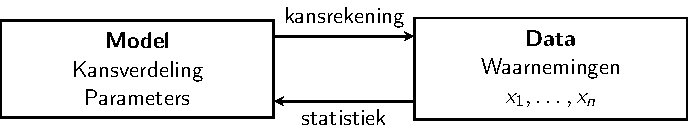
\includegraphics{../tikz/3_prob_vs_stat.pdf}
        \end{center}
        \vfill
        \begin{itemize}
            \item \textbf{Kansrekening:} het model is bekend, wat zien we in de data?
            \item \textbf{Statistiek:} de data is bekend, wat kunnen we zeggen over het model?
        \end{itemize}
    \end{frame}

    \begin{frame}{Populatie en steekproef}
        \begin{center}
            \begin{tabular}{lll}
                \toprule
                    & \textbf{Populatie} & \textbf{Steekproef} \\
                \midrule
                    Wat                & alle objecten van belang & een deelverzameling (grootte $n$) \\
                    Grootheden         & \concept{parameters} & \concept{statistieken} \\
                    Bekend?            & meestal niet & ja, berekend uit data \\
                \bottomrule
            \end{tabular}
        \end{center}
        \vfill
        \textbf{Doel:} aan de hand van \concept{steekproefdata} uitspraken doen over \concept{populatieparameters}.
    \end{frame}

    \begin{frame}{Voorbeeld: Defensie Conditie Proef}
        Op een willekeurige dag wordt van de militairen die aan de Defensie Conditie Proef (DCP) deelnemen de afstand gemeten die tijdens de 12 minutenloop wordt afgelegd.
        \vfill
        \begin{itemize}[<+->]\setlength\itemsep{2em}
            \item Met welk type kansvariabele (discreet of continu) hebben we te maken?
            \[ {\color{highlightcolor}\text{De afgelegde afstand $X$ is een continue variabele}}\]
            \item Wat is in dit geval de populatie en de steekproef?
                    \begin{itemize}
                        \color{highlightcolor}
                        \item \textbf{Populatie:} groep van alle militairen binnen Defensie
                        \item \textbf{Steekproef:} subgroep die vandaag de DCP doet.
                    \end{itemize} 
            \item Over welke populatieparameters willen we meer weten?
            \begin{itemize}
                \color{highlightcolor}
                \item Gemiddelde afgelegde afstand $\mu$ voor de gehele populatie.
                \item Fractie $p$ van militairen die hun leeftijdsnorm halen.
            \end{itemize} 
        \end{itemize}
    \end{frame}

    \begin{frame}{Een steekproef als kansvariabele}
        \textbf{Merk op:} op verschillende dagen bestaat de steekproef uit een andere subgroep, en 
        steekproefgemiddelden zullen dus ook verschillen!
        \vfill
        We onderscheiden een steekproef op twee manieren:
        \begin{itemize}[<+->]\setlength\itemsep{2em}
            \item \concept{Theoretische steekproef} (voordat de samenstelling is bepaald): een reeks \emph{onafhankelijke en gelijk verdeelde} kansvariabelen $X_1, X_2, \ldots, X_n$
            met $E(X_i) = \mu$ en $\sigma(X_i) = \sigma$.
            \item \concept{Geobserveerde steekproef} (nadat de samenstelling is bepaald):
            een reeks uitkomsten $x_1, x_2, \ldots, x_n$ van bovengenoemde kansvariabelen .
        \end{itemize}
    \end{frame}

    \begin{frame}{Schatter en schatting}
        \concept{Schatter} (\emph{estimator}): functie van een theoretische steekproef waarmee je een parameter $\theta$ kunt schatten.

        \concept{Schatting} (\emph{estimate}): een uitkomst van deze functie voor een geobserveerde steekproef.
        \vfill
        \begin{center}
            \begin{tabular}{lll}
                \toprule
                    \textbf{Parameter} & \textbf{Schatter} (kansvariabele) & \textbf{Schatting} (uitkomst) \\
                \midrule
                    $\mu$      & $\overline{X} = \frac{1}{n}\sum_{i=1}^n X_i$ & $\overline{x} = 12.5$ \\
                    $\sigma^2$ & $S^2 = \frac{1}{n-1}\sum_{i=1}^n (X_i - \overline{X})^2$ & $s^2 = 6$ \\
                    $p$        & $\hat{P} = \frac{\text{aantal successen}}{n}$ & $\hat{p} \approx 0.3871$ \\
                \bottomrule
            \end{tabular}
        \end{center}
        \vfill
        \textbf{Algemeen:} we schrijven vaak $\hat{\Theta}$ voor een schatter en $\hat{\theta}$ voor een schatting van een populatieparameter $\theta$.
    \end{frame}

    \begin{frame}{Verwachting en variantie van het steekproefgemiddelde}
        Dankzij lineariteit kunnen we de eigenschappen van $\overline{X}$ afleiden:
        \begin{align*}
            E(\overline{X}) &= E\left(\frac{1}{n}\sum_{i=1}^n X_i\right) = \frac{1}{n}\sum_{i=1}^n E(X_i) = \frac{1}{n} \cdot n \mu = \mu \\
            \Var{\overline{X}} &= \frac{1}{n^2}\sum_{i=1}^n \Var{X_i} = \frac{1}{n^2} \cdot n\sigma^2 = \frac{\sigma^2}{n}
        \end{align*}
        \vfill
        \begin{itemize}
            \item Gemiddeld genomen zit $\overline{X}$ op de juiste waarde $\mu$.
            \item Meer data $\Rightarrow$ kleinere spreiding: $\sigma(\overline{X}) = \frac{\sigma}{\sqrt{n}}$.
        \end{itemize}
    \end{frame}

%==================================================================
\section{Zuivere schatters en efficiëntie}
%==================================================================

    \begin{frame}{Wat is een goede schatter?}
        Voor een parameter $\theta$ zijn er vaak meerdere schatters mogelijk.
        \vfill
        Zo kun je het populatiegemiddelde $\mu$ schatten met:
        \begin{itemize}[<+->]
            \item $\overline{X}$ (het gemiddelde van alle $n$ metingen),
            \item $X_1$ (alleen de eerste meting),
            \item $\frac{X_1 + X_2}{2}$,
            \item de mediaan van de steekproef.
        \end{itemize}
        \vfill\pause
        \textbf{Welke is het beste, en hoe bepaal je dat?}
    \end{frame}

    \begin{frame}{Zuiverheid}
        Eerder zagen we dat schatters $\hat{\Theta}$ een functie zijn van een steekproef, oftewel een functie van kansvariabelen:
        \[
            \hat{\Theta} = g(X_1, X_2, X_3, \ldots, X_n).
        \] 

        De \concept{bias} van een schatter $\hat{\Theta}$ voor $\theta$ is
        \[
            \operatorname{Bias}(\hat{\Theta}) = E(\hat{\Theta}) - \theta.
        \]
        Een schatter is \concept{zuiver} (\emph{unbiased}) als $\operatorname{Bias}(\hat{\Theta}) = 0$, oftewel als
        $E(\hat{\Theta}) = \theta$.
        \vfill
        Een zuivere schatter zit \emph{gemiddeld} op de juiste waarde, niet noodzakelijk bij iedere steekproef.
    \end{frame}

    \begin{frame}{Voorbeeld: $\overline{X}$ is een zuivere schatter voor $\mu$}
        We zagen eerder al dat $E(\overline{X}) = \mu$, dus $\overline{X}$ is een zuivere schatter voor $\mu$.
        \vfill
        Ook de schatters $X_1$ en $\frac{X_1 + X_2}{2}$ zijn zuiver voor $\mu$, want
        \begin{itemize}[<+->]
            \item $E(X_1) = \mu$,
            \item $E\left(\frac{X_1 + X_2}{2}\right) = \frac{1}{2}E(X_1) + \frac{1}{2} E(X_2) = \frac{1}{2}\mu+\frac{1}{2}\mu= \mu$.
        \end{itemize}
        \vfill\pause
        \textbf{Zuiverheid alleen is dus niet genoeg om te kiezen.}
    \end{frame}

    \begin{frame}{Vergelijken van zuivere schatters}
        Als twee schatters beide zuiver zijn, kies degene met de \emph{kleinste variantie}.
        \vfill
        \begin{center}
            \includegraphics[width=0.9\textwidth]{./3_unbiased_estimators.png}
        \end{center}
        \vfill
        Een schatter met een kleine variantie heet \concept{efficiënt}: dit geeft ons meer vertrouwen dat een willekeurige schatting dichter bij de ware $\mu$ ligt.
    \end{frame}

    \begin{frame}{Voorbeeld: schatters voor $\mu$ vergelijken}
        Laat $X_1, \ldots, X_n$ onafhankelijk zijn met $E(X_i) = \mu$ en $\Var{X_i} = \sigma^2$.
        \vfill
        \begin{center}
            \begin{tabular}{lcc}
                \toprule
                    \textbf{Schatter} & \textbf{Verwachting} & \textbf{Variantie} \\
                \midrule
                    $X_1$ & $\mu$ & $\sigma^2$ \\
                    $\frac{X_1 + X_2}{2}$ & $\mu$ & $\frac{\sigma^2}{2}$ \\
                    $\overline{X}$ & $\mu$ & $\frac{\sigma^2}{n}$ \\
                \bottomrule
            \end{tabular}
        \end{center}
        \vfill
        Alledrie zijn zuiver, maar voor $n > 2$ geldt 
        \[
            \Var{\overline{X}} < \Var{\frac{X_1 + X_2}{2}} < \Var{X_1}.
        \]
        Het steekproefgemiddelde $\overline{X}$ is dus het meest efficiënt. 
    \end{frame}

    \begin{frame}{Tradeoff tussen zuiverheid en efficiëntie}
        Een schatter heeft idealiter beide eigenschappen, maar dit is niet altijd mogelijk.
        Een maat die hier rekening mee houdt is de \concept{gemiddelde kwadratische fout} (\emph{mean squared error}):
        \[
            \operatorname{MSE}(\hat{\Theta}) = E\left((\hat{\Theta} - \theta)^2\right) = \Var{\hat{\Theta}} + \operatorname{Bias}(\hat{\Theta})^2
        \]
        \begin{itemize}
            \item In sommige situaties hebben zuivere schatters een heel hoge variantie.
            \item Introduceren van een kleine bias tot kan drastische daling in variantie leiden
        \end{itemize}
    \end{frame}

    \begin{frame}{Voorbeeld: een zuivere schatter voor $\sigma$}
        De volgende schatter voor $\sigma^2$ is \concept{zuiver}:
        \[
            S^2 = \frac{1}{n-1}\sum_{i=1}^n (X_i - \overline{X})^2
        \]
        \vfill
        \textbf{Merk op:} we delen door $n-1$ en niet door $n$. 
        Dit komt omdat $\overline{X}$ op zichzelf al een schatting is uit de steekproef en daarmee per definitie \enquote{dichter bij}
        de data ligt dan het populatiegemiddelde $\mu$.
    \end{frame}

    \begin{frame}\frametitle{Afleiding: $E(S^2) = \sigma^2$}
        Gebruik $\sum_{i}(X_i - \mu)^2 = \sum_i (X_i - \overline{X})^2 + n(\overline{X} - \mu)^2$.\pause
        \vfill
        Neem verwachtingswaarden:
        \begin{align*}
            \underbrace{\sum_i E\left((X_i - \mu)^2\right)}_{\sum_i \Var{X_i}=n\sigma^2} &= E\left(\sum_i (X_i - \overline{X})^2\right) + n \cdot \underbrace{E\left((\overline{X} - \mu)^2\right)}_{\Var{\overline{X}} = \sigma^2/n}
        \end{align*}\pause
        Dus $E\left(\sum_i (X_i - \overline{X})^2\right) = n\sigma^2 - \sigma^2 = (n-1)\sigma^2$.\pause
        \vfill
        Hieruit volgt dat:
        \[
            E(S^2) = E\left(\frac{1}{n-1}\cdot \sum_i (X_i - \overline{X})^2\right)=\frac{1}{n-1}E\left(\cdot \sum_i (X_i - \overline{X})^2\right)=\sigma^2.
        \]
    \end{frame}

    % \begin{frame}{Maximum likelihood}
    %     % TODO: kies: weglaten, één slide (teaser), of verplaatsen naar een volgend college
    %     Hoe vind je een goede schatter als er geen voor de hand liggende formule is?
    %     \vfill
    %     \begin{itemize}
    %         \item \concept{Maximum likelihood}: kies de parameterwaarde waarvoor de waargenomen data het \emph{meest waarschijnlijk} is.
    %         \item Voor de normale verdeling levert dit $\overline{X}$ voor $\mu$.
    %     \end{itemize}
    % \end{frame}

    \begin{frame}{Oefening: schatters vergelijken}
        Laat $X_1, X_2, X_3$ onafhankelijk zijn met $E(X_i)=\mu$ en $\Var{X_i}=\sigma^2$. 
        \vfill
        Beschouw
        \begin{align*}
            \hat{\Theta}_A &= \frac{X_1 + X_2 + X_3}{3},\\
            \hat{\Theta}_B &= \frac{X_1 + 2X_2 + 3X_3}{6},\\
            \hat{\Theta}_C &= \frac{33X_1 + 33X_2 + 33X_3}{100}.
        \end{align*}
        \begin{enumerate}
            \item Welke schatters zijn zuiver voor $\mu$?
            \item Bereken de variantie van iedere schatter.
            \item Welke zuivere schatter is het meest efficiënt?
        \end{enumerate}
    \end{frame}

    \begin{frame}\frametitle{Uitwerking: schatters vergelijken}
        {\small
        \begin{align*}
            E(\hat{\Theta}_A) &= \frac{1}{3}E(X_1) + \frac{1}{3}E(X_2) + \frac{1}{3}E(X_3) = \mu. \\
            E(\hat{\Theta}_B) &= \frac{1}{6}E(X_1) + \frac{1}{3}E(X_2) + \frac{1}{2}E(X_3) = \mu. \\
            E(\hat{\Theta}_C) &= \frac{1}{4}E(X_1) + \frac{1}{4}E(X_2) + \frac{1}{4}E(X_3) = \frac{3}{4}\mu.
        \end{align*}
        Alleen schatters $\hat{\Theta}_A$ en $\hat{\Theta}_B$ zijn dus zuiver.
        \begin{align*}
            \Var{\hat{\Theta}_A} &= \frac{3\sigma^2}{9} = \frac{\sigma^2}{3} \approx 0.333\sigma^2, \\
            \Var{\hat{\Theta}_B} &= \frac{(1+4+9)\sigma^2}{36} = \frac{7\sigma^2}{18} \approx 0.389\sigma^2,\\
            \Var{\hat{\Theta}_C} &= \frac{3\cdot (1)\sigma^2}{16} = \frac{3\sigma^2}{16} \approx 0.1875\sigma^2.
        \end{align*}
        Van de zuivere schatters is $\hat{\Theta}_A$ (het gemiddelde) het meest efficiënt (de onzuivere
        schatter $\hat{\Theta}_C$ heeft de kleinste variantie).
        }
    \end{frame}

    %==================================================================
    \section{Betrouwbaarheidsintervallen: $\sigma$ bekend}
    %==================================================================

    \begin{frame}{Voorbeeld: de Defensie ConditieProef}
        Op een willekeurige dag nemen $50$ militairen deel aan de 12-minutenloop van de Defensie ConditieProef
        en leggen daarbij gemiddeld $\overline{x}=2418.6$ meter af.
        Neem aan dat de \concept{populatie}standaardafwijking $\sigma = 75.2$ is.
        \vfill
        \begin{itemize}[<+->]\setlength\itemsep{1em}
            \item Is het \concept{populatie}gemiddelde $\mu$ gelijk aan $2418.6$ meter? 
            \item \emph{Waarschijnlijk niet, dit is slechts een schatting!
            Als morgen een nieuwe steekproef van militairen deelneemt aan de 12-minutenloop,
            zal het steekproefgemiddelde weer net iets anders zijn.}
        \end{itemize}
        \vfill
        \only<3->{
            \textbf{Wat kunnen we dan wel zeggen over het populatiegemiddelde $\mu$?}
        }
    \end{frame}

    \begin{frame}{Omschrijven naar de standaardnormale verdeling}
        Vanwege de centrale limietstelling kunnen we steekproefgemiddelden koppelen aan $\mu$:
        \[
            \overline{X} \sim N\left(\mu, \frac{\sigma}{\sqrt{n}}\right)
        \]
        \vfill\pause
        Standaardiseren geeft de \concept{standaardnormale verdeling}:
        \[
            Z = \frac{\overline{X} - \mu}{\sigma / \sqrt{n}} \sim N(0, 1).
        \]
        \vfill\pause
        \textbf{Voordeel:} de kansverdeling van $Z$ is volledig bekend, die van $\overline{X}$ niet (want $\mu$ is onbekend!)
    \end{frame}

    \begin{frame}{Wat zijn \enquote{redelijke uitkomsten} voor $N(0,1)$?}
        \pause
        \only<2>{
            Stel $\alpha \in (0,1)$, bv. $\alpha = 0.05$.
            \vfill
            Met kans $1 - \alpha = 0.95$ krijgen we een uitkomst tussen de grenswaarden op
            $\alpha/2=0.025$ en $1-\alpha/2=0.975$ van de verdeling:
        }
        \only<2->{
            \begin{center}
                \includegraphics[width=0.7\textwidth]{3_prediction_interval_z.png}
            \end{center}
        }
        \only<3>{
            We noteren met $z_{\alpha/2}$ de grenswaarde op $1-\alpha/2$ van de verdeling:
            \[
                z_{{\alpha/2}} = \invnorm(\opp=1-\alpha/2, \mu=0, \sigma=1)
            \]
            $N(0,1)$ is symmetrisch rond $0$, dus de grenswaarden zijn $-z_{\alpha/2}$ en $z_{\alpha/2}$.
        }
    \end{frame}

    \begin{frame}{Intervalschatting voor $\mu$}
        Wiskundig samengevat geeft dit:
        \[
            P\left(-z_{\alpha/2} \leq \frac{\overline{X} - \mu}{\sigma / \sqrt{n}} \leq z_{\alpha/2}\right) = 1 - \alpha.
        \]
        \vfill\pause
        Herschrijven zodat alleen $\mu$ in het midden staat:
        \[
            P\left(\overline{X} - z_{\alpha/2}\cdot\frac{\sigma}{\sqrt{n}} \leq \mu \leq \overline{X} + z_{\alpha/2}\cdot\frac{\sigma}{\sqrt{n}}\right) = 1 - \alpha.
        \]
    \end{frame}

    \begin{frame}{Betrouwbaarheidsinterval voor $\mu$ ($\sigma$ bekend)}
        Een $100 \cdot (1-\alpha) \%$-\concept{betrouwbaarheidsinterval} voor $\mu$ is
        \[
            \left[\overline{X} - z_{\alpha/2} \cdot \frac{\sigma}{\sqrt{n}}, \quad \overline{X} + z_{\alpha/2} \cdot \frac{\sigma}{\sqrt{n}}\right]
        \]
        \vfill
        \begin{itemize}
            \item $\overline{X}$: steekproefgemiddelde (\textbf{schatter, dus kansvariabele!})
            \item $\pm z_{\alpha/2}$: kritieke $z$-waarden.
            \item $z_{\alpha/2} \cdot \frac{\sigma}{\sqrt{n}}$: de \concept{foutmarge}
        \end{itemize}
        \vfill\pause
        \textbf{Merk op:} de grenzen van een betrouwbaarheidsinterval zijn opnieuw kansvariabelen.
        Verschillende steekproeven geven verschillende intervalgrenzen!
    \end{frame}

    \begin{frame}{Voorbeeld: de Defensie ConditieProef}
        Op een willekeurige dag nemen $64$ militairen deel aan de 12-minutenloop van de Defensie ConditieProef
        en leggen daarbij gemiddeld $\overline{x}=2418.6$ meter af.
        Neem aan dat de \concept{populatie}standaardafwijking $\sigma = 75.2$ is.
        \vfill
        \textbf{Bepaal een \SI{95}{\percent}-betrouwbaarheidsinterval voor het gemiddelde $\mu$.}
        \pause\vfill
        {\color{highlightcolor}
        We willen een \SI{95}{\percent}-betrouwbaarheidsinterval, dus $\alpha = 0.05$.

        Dat betekent dat
        \[
            z_{\alpha/2} = \invnorm(\opp=1-\alpha/2=0.975, \mu=0, \sigma=1) \approx 1.9600.
        \]
        Invullen van $\overline{x}=2418.6$ meter en $\sigma=75.2$ meter geeft:
        \[
            \overline{x} \pm z_{\alpha/2} \cdot \frac{\sigma}{\sqrt{n}} = 2418.6 \pm 1.960 \cdot \frac{75.2}{\sqrt{64}} \Rightarrow [2400.176, 2437.024] \text{ meter.}
        \]}
    \end{frame}

    \begin{frame}{Stellingen (waar / niet waar)}
        \only<1,2>{
            \textbf{Stelling 1:} $\mu$ ligt met \SI{95}{\percent} kans tussen $2400.176$ en $2437.024$.
        }
        \only<2>{
            \vfill
            {
                \color{highlightcolor} NIET WAAR: de echte waarde van $\mu$ staat vast (ook al is deze waarde onbekend).
                Er is dus geen sprake van kans: $\mu$ ligt wel of niet in het berekende interval $[2400.176, 2437.024]$.
                Bij herhaalde steekproeven zal \SI{95}{\percent} van de berekende intervallen de echte waarde van $\mu$ bevatten.
            }
        }
        \only<3,4>{
            \textbf{Stelling 2:} als de steekproefgrootte $n$ verdubbelt, wordt het interval half zo breed.
        }
        \only<4>{
            \vfill
            {
                \color{highlightcolor} NIET WAAR: de intervalbreedte is proportioneel met $\frac{1}{\sqrt{n}}$. 
                Als $n$ verdubbelt, dan wordt het interval dus $\frac{1}{\sqrt{2}} = \frac{1}{2}\sqrt{2}$ keer zo breed.
            }
        }
        \only<5,6>{
            \textbf{Stelling 3:} Een \SI{99}{\percent}-betrouwbaarheidsinterval is breder dan een \SI{95}{\percent}-betrouwbaarheidsinterval berekend op dezelfde dataset.
        }
        \only<6>{
            \vfill
            {
                \color{highlightcolor} WAAR: hoe meer betrouwbaarheid we eisen dat een interval de werkelijke waarde van $\mu$ bevat,
                hoe breder het interval moet zijn.
            }
        }
    \end{frame}

    \begin{frame}{Wat zegt een specifiek interval ons nu daadwerkelijk?}
        Het betrouwbaarheidsinterval voor $\mu$ berekend voor deze specifieke steekproef van militairen loopt van $2400.176$ meter tot $2437.024$ meter.
        \vfill
        \begin{itemize}[<+->]\setlength\itemsep{2.5em}
            \item We weten dus niet of $\mu$ daadwerkelijk in dit interval ligt.
            \item Bij herhaaldelijk trekken van steekproeven zal in \SI{95}{\percent} van de gevallen het interval de echte $\mu$ bevatten.
            \item We hebben dus een statistische schattingsmethode die met een hoge mate van \concept{betrouwbaarheid} tot een interval leidt dat $\mu$ bevat.
        \end{itemize}
    \end{frame} 

    

    \begin{frame}{Demonstratie: betrouwbaarheidsintervallen}
        \begin{center}
            % TODO: link naar interactieve app
            \Large https://interactive-ci-n.streamlit.app/
        \end{center}
    \end{frame}

    \begin{frame}{Wat bepaalt de breedte van een betrouwbaarheidsinterval?}
        De breedte van een betrouwbaarheidsinterval is als volgt:
        \begin{align*}
            \text{breedte}  &= \text{rechtergrens} - \text{linkergrens} \\
                            &= \left(\overline{X} + z_{\alpha/2} \cdot \frac{\sigma}{\sqrt{n}}\right) - \left(\overline{X} - z_{\alpha/2} \cdot \frac{\sigma}{\sqrt{n}}\right) \\
                            &= 2 \cdot z_{\alpha/2} \cdot \frac{\sigma}{\sqrt{n}}
        \end{align*}
        \vfill\pause
        De breedte hangt dus af van drie dingen:
        \begin{itemize}[<+->]\setlength\itemsep{1em}
            \item Grotere $n$ $\Rightarrow$ smaller interval (meer data is meer nauwkeurigheid)
            \item Grotere $\sigma$ $\Rightarrow$ breder interval (meer spreiding is minder nauwkeurigheid)
            \item Kleinere $\alpha$ $\Rightarrow$ breder interval (meer betrouwbaarheid).
        \end{itemize}
    \end{frame}

    \begin{frame}{Hoe groot moet de steekproef zijn?}
        De foutmarge binnen een betrouwbaarheidsinterval is $\pm z_{\alpha/2} \cdot \frac{\sigma}{\sqrt{n}}$.

        Bij een gewenste maximale foutmarge $\pm E$ moet dus gelden:
        \[
            z_{\alpha/2} \cdot \frac{\sigma}{\sqrt{n}} \leq E \quad \Rightarrow \quad n \geq \left(\frac{z_{\alpha/2} \cdot \sigma}{E}\right)^2
        \]
        \vfill\pause
        \textbf{Voorbeeld:} $\sigma = 75.2$, foutmarge $\pm E = \pm 10$ meter, $\alpha = 0.05$
        \[
            n \geq \left(\frac{z_{\alpha/2} \cdot \sigma}{E}\right)^2 = \left(\frac{1.9600 \cdot 75.2}{10}\right)^2 \approx 217.2360.
        \]
        \vfill\pause
        Hoe groter de $n$, hoe kleiner de foutmarge, dus rond af \emph{naar boven}:
        \[
            n \geq 218.
        \]
    \end{frame}

    % \begin{frame}{Oefening: betrouwbaarheidsintervallen ($\sigma$ bekend)}
    %     De diepgang van een amfibisch landingsvaartuig wordt gemeten. Uit eerdere metingen is bekend dat $\sigma = 0.15$ m.
    %     \vfill
    %     \begin{enumerate}
    %         \item Bij $n = 25$ metingen is $\overline{x} = 1.32$ m. Bepaal een \SI{90}{\percent}-, \SI{95}{\percent}- en \SI{99}{\percent}-betrouwbaarheidsinterval voor $\mu$.
    %         \item Wat gebeurt er met de breedte bij hoger niveau?
    %         \item Hoeveel metingen zijn nodig voor een \SI{95}{\percent}-interval met foutmarge hooguit $0.03$ m?
    %     \end{enumerate}
    %     % Antwoorden: 1) 1.32 +- 1.645*0.03 -> [1.271, 1.369]; 1.32 +- 1.960*0.03 -> [1.261, 1.379]; 1.32 +- 2.576*0.03 -> [1.243, 1.397]
    %     % 3) n >= (1.96*0.15/0.03)^2 = 96.04 -> 97
    % \end{frame}

%==================================================================
\section{Betrouwbaarheidsintervallen: $\sigma$ onbekend}
%==================================================================
    % Vervolg op de frames over het betrouwbaarheidsinterval met bekende sigma.
    % Gebruikt dezelfde macro's als jouw deck: \concept, \SI, highlightcolor.
    % Plaats dit blok na het frame "Hoe groot moet de steekproef zijn?".

    \begin{frame}{Wat als ook de populatiestandaardafwijking $\sigma$ onbekend is?}
        \textbf{Idee:} vervang $\sigma$ door de \concept{steekproef}standaardafwijking
        \[
            S = \sqrt{\frac{1}{n-1}\sum_{i=1}^{n} \left(X_i - \overline{X}\right)^2},
        \]
        en neem het interval
        \[
            \left[\overline{X} - z_{\alpha/2} \cdot \frac{S}{\sqrt{n}}, \quad \overline{X} + z_{\alpha/2} \cdot \frac{S}{\sqrt{n}}\right]
        \]
        \vfill\pause
        De schatter $S$ is echter zelf ook een kansvariabele, daardoor geldt:
        \[
            \frac{\overline{X} - \mu}{S / \sqrt{n}} \text{ is \emph{\textbf{niet}} standaardnormaal verdeeld.}
        \]
        We kunnen dus niet zomaar $\pm z_{\alpha/2}$ gebruiken.
    \end{frame}

    \begin{frame}{De $t$-verdeling}
        Omdat de schatter $S$ zelf een kansvariabele is, zit er nog meer onzekerheid in de voorspellende waarde van een intervalschatter.
        \vfill
        Er geldt wel dat
        \[
            T = \frac{\overline{X} - \mu}{S / \sqrt{n}} \sim t(\df=n-1),
        \]
        de \concept{$t$-verdeling} met $\df=n-1$ \concept{vrijheidsgraden} (\emph{degrees of freedom}).
    \end{frame}

    \begin{frame}{De $t$-verdeling}
        De $t$-verdeling lijkt op de standaardnormale verdeling $N(0,1)$:
        \vfill
        \begin{itemize}[<+->]\setlength\itemsep{2.5em}
            \item Ook symmetrisch rond gemiddelde $0$.
            \item Zwaardere \enquote{staarten}: extremere uitkomsten zijn waarschijnlijker door de extra onzekerheid in de spreiding.
            \item Voor grotere $n$ lijkt $t(\df=n-1)$ steeds meer op $N(0,1)$.
        \end{itemize}
    \end{frame}

    \begin{frame}{Demonstratie: de $t$-verdeling}
        \begin{center}
            \Large https://interactive-t.streamlit.app
        \end{center}
    \end{frame}

    \begin{frame}{Wat zijn \enquote{redelijke uitkomsten} voor $t(\df=n-1)$?}
        \pause
        \only<2>{
            Stel $\alpha \in (0,1)$, bv. $\alpha = 0.05$.
            \vfill
            Met kans $1 - \alpha = 0.95$ krijgen we een uitkomst tussen de grenswaarden op
            $\alpha/2=0.025$ en $1-\alpha/2=0.975$ van de verdeling:
        }
        \only<2->{
            \begin{center}
                \includegraphics[width=0.7\textwidth]{3_prediction_interval_t.png}
            \end{center}
        }
        \only<3>{
            We noteren met $t_{n-1,\alpha/2}$ de grenswaarde op $1-\alpha/2$ van de verdeling:
            \[
                t_{{n-1,\alpha/2}} = \invt(\opp=1-\alpha/2, \df=n-1)
            \]
            $t(\df=n-1)$ is symmetrisch rond $0$, dus de grenswaarden zijn $\pm t_{n-1,\alpha/2}$.
        }
    \end{frame}

    \begin{frame}{Intervalschatting voor $\mu$}
        Wiskundig samengevat geeft dit:
        \[
            P\left(-t_{n-1,\alpha/2} \leq \frac{\overline{X} - \mu}{S / \sqrt{n}} \leq t_{n-1,\alpha/2}\right) = 1 - \alpha.
        \]
        \vfill\pause
        Herschrijven zodat alleen $\mu$ in het midden staat:
        \[
            P\left(\overline{X} - t_{n-1,\alpha/2}\cdot\frac{S}{\sqrt{n}} \leq \mu \leq \overline{X} + t_{n-1,\alpha/2}\cdot\frac{S}{\sqrt{n}}\right) = 1 - \alpha.
        \]
    \end{frame}

    \begin{frame}{Betrouwbaarheidsinterval voor $\mu$ ($\sigma$ onbekend)}
        Een $100 \cdot (1-\alpha) \%$-betrouwbaarheidsinterval voor $\mu$ is
        \[
            \left[\overline{X} - t_{n-1,\alpha/2} \cdot \frac{S}{\sqrt{n}}, \quad \overline{X} + t_{n-1,\alpha/2} \cdot \frac{S}{\sqrt{n}}\right]
        \]
        \vfill
        \begin{itemize}
            \item $S$: steekproefstandaardafwijking (\textbf{schatter, dus kansvariabele!})
            \item $\pm t_{n-1,\alpha/2}$: kritieke $t$-waarden
            \item $t_{n-1,\alpha/2} \cdot \frac{S}{\sqrt{n}}$: de \concept{foutmarge}
        \end{itemize}
    \end{frame}

    \begin{frame}{Voorbeeld: de Defensie ConditieProef ($\sigma$ onbekend)}
        Op een willekeurige dag nemen $25$ militairen deel aan de 12-minutenloop van de Defensie ConditieProef
        en leggen daarbij gemiddeld $\overline{x}=2418.6$ meter af, met steekproefstandaardafwijking $s = 75.2$ meter.
        De populatie is bij benadering normaal verdeeld.
        \vfill
        \textbf{Bepaal een \SI{95}{\percent}-betrouwbaarheidsinterval voor het gemiddelde $\mu$.}
        \pause\vfill
        {\color{highlightcolor}
        Hier is $\alpha = 0.05$ en $\df=n - 1 = 24$ vrijheidsgraden, dus $t_{24,0.025} \approx 2.0639$.

        Invullen geeft:
        \[
            \overline{x} \pm t_{n-1,\alpha/2} \cdot \frac{s}{\sqrt{n}} = 2418.6 \pm 2.0639 \cdot \frac{75.2}{\sqrt{25}} \Rightarrow [2387.5589, 2449.6410] \text{ meter.}
        \]}
    \end{frame}

    \begin{frame}{Wat als we toch $z_{\alpha/2}$ hadden gebruikt?}
        \textbf{Berekende interval met $t$-verdeling:} $[2387.5589, 2449.6410]$ \text{ meter.}
        \vfill
        Met $z_{0.025} = 1.9600$ in plaats van $t_{24,0.025} = 2.0639$:
        \[
            2418.6 \pm 1.9600 \cdot \frac{75.2}{\sqrt{25}} \Rightarrow [2389.1221, 2448.0779] \text{ meter.}
        \]
        \vfill\pause
        Dit interval is te smal: bij kleine $n$ houdt het geen rekening met de onzekerheid in $S$.
    \end{frame}

    \begin{frame}{Stellingen (waar / niet waar)}
        \only<1,2>{
            \textbf{Stelling 1: } bij onbekende $\sigma$ en kleine $n$ mag je gewoon $z_{\alpha/2}$ gebruiken.
        }
        \only<2>{
            \vfill
            \color{highlightcolor} NIET WAAR: de dekking is dan lager dan de beoogde $100 \cdot (1-\alpha)\%$. Gebruik $t_{n-1,\alpha/2}$.
        }
        \only<3,4>{
            \textbf{Stelling 2: } de breedte van het interval is bij onbekende $\sigma$ een vaste waarde, zodra $n$ en $\alpha$ gekozen zijn.
        }
        \only<4>{
            \vfill
            \color{highlightcolor} NIET WAAR: $S$ verschilt per steekproef, dus de breedte $2 \cdot t_{n-1,\alpha/2} \cdot S/\sqrt{n}$ is zelf een kansvariabele.
        }
        \only<5,6>{
            \textbf{Stelling 2: } Voor grote $n$ zijn $t_{n-1,\alpha/2}$ en $z_{\alpha/2}$ bijna gelijk.
        }
        \only<6>{
            \vfill
            \color{highlightcolor} WAAR. In de limiet geldt dat 
            \[\lim_{n\to\infty} t(\df=n-1) \to N(0,1).\]
        }
    \end{frame}

    \begin{frame}{Hoe groot moet de steekproef zijn als $\sigma$ onbekend is?}
        De breedte van een betrouwbaarheidsinterval voor $\mu$ ($\sigma$ onbekend) is
        \begin{align*}
            \text{breedte} = 2 \cdot t_{n-1,\alpha/2} \cdot \frac{S}{\sqrt{n}}
        \end{align*}
        \vfill\pause
        Omdat $S$ een kansvariabele is, hebben we geen gesloten formule voor de minimaal benodigde $n$ om een betrouwbaarheidsinterval met foutmarge $\pm E$ te behalen.
        Hiervoor gebruiken we de volgende aanpak:
        \vfill
        \begin{enumerate}[<+->]\setlength\itemsep{1em}
            \item Schat $\sigma$ met $s$ op basis van een steekproef.
            \item Gebruik de eerdere formule $n \geq \left( \frac{z_{\alpha/2} \cdot \sigma}{E} \right)^2$ met \enquote{$\sigma = s$}.
            \item Vul waarden voor $n$ in de uitdrukking $2 \cdot t_{n-1,\alpha/2} \cdot \frac{s}{\sqrt{n}}$ in (startend bij berekende $n$)
            \item Kijk voor welke $n$ de uitdrukking voor het eerst kleiner dan $E$ is.
        \end{enumerate}
    \end{frame}

    \begin{frame}{Oefening}
        \only<1>{
            Op een willekeurige dag nemen $12$ militairen deel aan de 12-minutenloop van de Defensie ConditieProef
            en leggen daarbij gemiddeld $\overline{x}=2395.4$ meter af met een steekproefstandaardafwijking $s = 84.6$ meter.
            \vfill
        }
        \begin{enumerate}
            \item Bepaal een \SI{90}{\percent}-betrouwbaarheidsinterval voor $\mu$.
            \item Uitgaande van dezelfde $\overline{x}$ en $s$, wat zou de minimale steekproefgrootte $n$ zijn waarvoor het \SI{90}{\percent}-betrouwbaarheidsinterval voor $\mu$ een foutmarge van $\pm 10$ meter heeft.
        \end{enumerate}
    \end{frame}

    \begin{frame}{Uitwerking}
        \textbf{Bepaal een \SI{90}{\percent}-betrouwbaarheidsinterval voor $\mu$.}
        \pause\vfill
        {\color{highlightcolor}
            We hebben te maken met een \SI{90}{\percent}-betrouwbaarheidsinterval, dus $\alpha=0.10$. 
            Verder is $n = 12$, dus de kritieke $t$-waarde is
            \[
                t_{11,0.05} = \invt(\opp=1-\alpha/2=0.95, \df=n-1=11) \approx 1.7959.
            \]
            Het \SI{90}{\percent}-betrouwbaarheidsinterval voor $\mu$ is dus
            \[
                2395.4 \pm 1.7959 \cdot \frac{84.6}{\sqrt{12}} \Rightarrow [2351.5411, 2439.2589].
            \]
        }
    \end{frame}

    \begin{frame}{Uitwerking}
        \textbf{Bepaal de minimale steekproefgrootte $n$ waarvoor een \SI{90}{\percent}-betrouwbaarheidsinterval voor $\mu$ een foutmarge van $\pm 10$ meter heeft.}
        \pause\vfill
        {
            \begin{itemize}[<+->]
                \color{highlightcolor}
                \item Als $\alpha = 0.10$, dan is $z_{\alpha/2} \approx 1.6449$.
                \item Als richtwaarde voor $n$ gebruiken we de formule alsof $\sigma$ bekend is:
                \[ n \geq \left( \frac{z_{\alpha/2} \cdot \sigma}{E} \right)^2 = \left( \frac{1.6449 \cdot 84.6}{10} \right)^2 \approx 193.6401 \Rightarrow 194 \]
                \item Vul waarden voor $n$ in de uitdrukking $2 \cdot \invt(0.95, n-1) \cdot \frac{84.6}{\sqrt{n}}$ in:
                \begin{align*}
                    n = 195 &\Rightarrow y_1 = 2 \cdot \invt(0.95, 195-1) \cdot \frac{84.6}{\sqrt{195}} \approx 10.013 > 10 \\
                    n = 196 &\Rightarrow y_1 = 2 \cdot \invt(0.95, 196-1) \cdot \frac{84.6}{\sqrt{196}} \approx 9.9871 < 10
                \end{align*}
                \item De minimale steekproefgrootte waarvoor het interval een foutmarge van hoogstens $\pm 10$ meter heeft is $n = 196$.
            \end{itemize}
        }
    \end{frame}

    \begin{frame}{Vergelijking: $\sigma$ bekend versus onbekend}
        \begin{center}
            \begin{tabular}{lll}
                \toprule
                    & \textbf{$\sigma$ bekend} & \textbf{$\sigma$ onbekend} \\
                \midrule
                    Spreiding         & $\sigma$ & $s$ (schatting) \\
                    Verdeling         & $N(0,1)$ & $t(\df=n-1)$ \\
                    Kritieke waarde   & $z_{\alpha/2}$ & $t_{\alpha/2, n-1}$ \\
                    Interval          & $\overline{X} \pm z_{\alpha/2}\cdot\frac{\sigma}{\sqrt{n}}$ & $\overline{X} \pm t_{\alpha/2,\, n-1}\cdot\frac{S}{\sqrt{n}}$ \\
                    Rekenmachine      & $\invnorm$ & $\invt$ \\
                \bottomrule
            \end{tabular}
        \end{center}
    \end{frame}

    %==================================================================
    \section{Hypothesetoetsen: deel 1}
    %==================================================================

    % NB: dit blok is het buffer-blok. Bij tijdsnood: reduceer tot de slides
    % "Idee", "Hypothesen", "Verband met betrouwbaarheidsintervallen".
    % Hypothesetoetsen, herschreven in dezelfde stijl als de betrouwbaarheidsintervallen:
%  - zelfde opbouw (standaardiseren -> kritiek gebied -> voorbeeld -> stellingen -> oefening)
%  - zelfde notatie (z_{\alpha}, t_{n-1,\alpha}, \overline{X}, S) en dezelfde voorbeeldcontext
%    (Defensie ConditieProef) in plaats van Boxer en pantserplaat
%  - rechtszaakmetafoor: H_0 = onschuldpresumptie, H_1 = bewering van de aanklager
% Vereist dezelfde macro's als de rest van het deck: \concept, \invnorm, \SI, highlightcolor.
% Vervangt alles vanaf het frame "Van schatten naar beslissen" tot en met "Oefening: hypothesetoetsen".

    \begin{frame}{Van schatten naar toetsen}
        De commandant beweert dat de gemiddelde afstand die militairen in de 12-minutenloop van de Defensie ConditieProef afleggen \emph{hoger} is dan de norm van $2400$ meter.
        Op een willekeurige dag nemen $64$ militairen deel en leggen daarbij gemiddeld $\overline{x}=2418.6$ meter af.
        Neem aan dat de \concept{populatie}standaardafwijking $\sigma = 75.2$ is.
        \vfill
        \begin{itemize}[<+->]\setlength\itemsep{1em}
            \item Is dit verschil met $2400$ meter toeval, of kunnen we echt zeggen dat het populatiegemiddelde $\mu > 2400$?
            \item Met een \concept{betrouwbaarheidsinterval} kun je de waarde van $\mu$ \emph{schatten}.
            \item Met een \concept{hypothesetoets} kun je een bewering over $\mu$ \emph{toetsen}.
        \end{itemize}
    \end{frame}

    \begin{frame}{Metafoor: rechtszaak}
        \renewcommand{\arraystretch}{1.5}
        \begin{center}
            \begin{tabular}{m{0.4\textwidth} m{0.46\textwidth}}
                \toprule
                    \textbf{Hypothesetoets} & \textbf{Rechtszaak} \\ 
                \midrule
                    \uncover<2->{\concept{Nulhypothese $H_0$} & Onschuld                    (status-quo)                } \\
                    \uncover<3->{\concept{Alternatieve hypothese $H_1$} & Schuld            (wel een effect)             } \\
                    \uncover<4->{\concept{Steekproefdata} & Dossier (verklaringen, DNA, $\ldots$)                       } \\
                    \uncover<5->{\concept{Significantieniveau $\alpha$} & Bewijsdrempel                                 } \\
                    \uncover<6->{\concept{Toetsingsgrootheid} & Kwantitatieve maat van bewijs                           } \\
                    \uncover<7->{\concept{Toetsuitslag} \newline ($H_0$ verwerpen of niet) & Vonnis (schuld / onschuld)} \\
                \bottomrule
            \end{tabular}
        \end{center}
        \vfill
        \only<8->{
            \textbf{Let op:} er is een verschil tussen \enquote{$H_0$ verwerpen} en \enquote{$H_0$ is niet waar}!
        }
    \end{frame}

    \begin{frame}{Nul- en alternatieve hypothese}
        We toetsen een bewering over het populatiegemiddelde $\mu$ ten opzichte van een vaste waarde $\mu_0$ (bijvoorbeeld de norm $\mu_0 = 2400$ meter).
        De alternatieve hypothese is daarbij de bewering die we willen toetsen.
        Er zijn drie soorten hypothesetoetsen voor het gemiddelde $\mu$:
        \vfill
        \begin{center}
            \renewcommand{\arraystretch}{1.4}
            \begin{tabular}{lll}
                \textbf{Type $H_1$} & & \textbf{Voorbeeld} \\ \hline
                Rechtszijdig & $\mu > \mu_0$ & de gemiddelde afstand is hoger dan $\mu_0$ \\
                Linkszijdig & $\mu < \mu_0$ & de gemiddelde afstand is lager dan $\mu_0$\\
                Tweezijdig & $\mu \neq \mu_0$ & de gemiddelde afstand wijkt af van $\mu_0$
            \end{tabular}
        \end{center}
        \vfill\pause
        \textbf{Merk op:} net als in de rechtbank behouden we $H_0$ tenzij de data sterk tegen $H_0$ pleit. De bewijslast ligt bij $H_1$.
    \end{frame}

    \begin{frame}{Omschrijven naar de standaardnormale verdeling}
        Bij een hypothesetoets nemen we altijd als startpunt aan dat $H_0$ waar is, dus $\mu = \mu_0$.
        Dan geldt:
        \[
            \overline{X} \sim N\left(\mu_0, \frac{\sigma}{\sqrt{n}}\right).
        \]
        \vfill\pause
        Standaardiseren geeft de \concept{toetsingsgrootheid}
        \[
            Z = \frac{\overline{X} - \mu_0}{\sigma / \sqrt{n}} \sim N(0, 1).
        \]
    \end{frame}

    \begin{frame}{Wat is \enquote{te extreem} onder $H_0$?}
        Het \concept{significantieniveau} $\alpha \in (0,1)$ bepaalt de grens tussen \enquote{extreme} en \enquote{niet-extreme} waarden voor de toetsingsgrootheid $Z$.
        \vfill
        Bewijs tegen $H_0$ is overtuigend als de toetsingsgrootheid in het \concept{kritieke gebied} ligt (de verzameling van extreme uitkomsten).
        \vfill
        \only<2>{
            \begin{center}
                \includegraphics[width=0.95\textwidth]{./3_linkszijdig.png}\\
                \textbf{Kritiek gebied: $Z = (-\infty, -z_{\alpha})$}
            \end{center}
        }
        \only<3>{
            \begin{center}
                \includegraphics[width=0.95\textwidth]{./3_tweezijdig.png}\\
                \textbf{Kritiek gebied: $Z = (-\infty, -z_{\alpha/2}) \cup (z_{\alpha/2}, \infty)$}
            \end{center}
        }
        \only<4>{
            \begin{center}
                \includegraphics[width=0.95\textwidth]{./3_rechtszijdig.png}\\
                \textbf{Kritiek gebied: $Z = (z_{\alpha}, \infty)$}
            \end{center}
        }
    \end{frame}

    \begin{frame}{De $p$-waarde}
        Een tweede manier om een toetsuitslag te bepalen is de \concept{$p$-waarde}.
        
        Dit is, \emph{onder $H_0$}, de kans op een uitkomst \textbf{minstens zo extreem} als de waargenomen toetsingsgrootheid $z$.
        \only<2>{
            \begin{center}
                \includegraphics[width=0.95\textwidth]{./3_linkszijdig_P.png}\\
                \textbf{$p$-waarde:} $p = P(Z \leq z)$ \\
                Verwerp $H_0$ indien $p < \alpha$
            \end{center}
        }
        \only<3>{
            \begin{center}
                \includegraphics[width=0.95\textwidth]{./3_tweezijdig_P.png}\\
                \textbf{$p$-waarde:} minimum van $P(Z \leq z)$ en $P(Z \geq z)$\\
                Verwerp $H_0$ indien $p < \alpha / 2$
            \end{center}
        }
        \only<4>{
            \begin{center}
                \includegraphics[width=0.95\textwidth]{./3_rechtszijdig_P.png}\\
                \textbf{$p$-waarde:} $p = P(Z \geq z)$ \\
                Verwerp $H_0$ indien $p < \alpha$
            \end{center}
        }
    \end{frame}

    \begin{frame}{Een hypothesetoets in zes stappen}
        \begin{enumerate}[<+->]\setlength\itemsep{1em}
            \item Formuleer $H_0$ en $H_1$.
            \item Kies het significantieniveau $\alpha$.
            \item Verzamel steekproefgegevens voor de toetsingsgrootheid.
            \item Bereken de toetsingsgrootheid.
            \item Bepaal de toetsuitslag met het kritieke gebied of de $p$-waarde (verwerp $H_0$ of niet).
            \item Vertaal de toetsuitslag naar de originele probleemcontext.
        \end{enumerate}
    \end{frame}

    \begin{frame}{Voorbeeld: de Defensie ConditieProef ($\sigma$ bekend)}
        Op een willekeurige dag nemen $64$ militairen deel aan de 12-minutenloop van de Defensie ConditieProef
        en leggen daarbij gemiddeld $\overline{x}=2418.6$ meter af.
        Neem aan dat de \concept{populatie}standaardafwijking $\sigma = 75.2$ is.
        \vfill
        \textbf{Toets bij $\alpha = 0.05$ of het gemiddelde hoger is dan de norm van $2400$ meter.}
    \end{frame}

    \begin{frame}{Voorbeeld: de Defensie ConditieProef ($\sigma$ bekend)}
        \textbf{Stap 1: formuleer $H_0$ en $H_1$}

        De uitspraak die we willen toetsen is of $\mu > 2400$, dus
        \[
            H_0: \mu \leq 2400 \text{ versus } H_1: \mu > 2400
        \]
        \vfill\pause
        \textbf{Stap 2: kies het significantieniveau}

        Het significantieniveau is in de vraag gegeven: $\alpha = 0.05$.
        \vfill\pause
        \textbf{Stap 3: verzamel steekproefgegevens voor de toetsingsgrootheid.}

        Ook de steekproefgegevens zijn in de vraag gegeven: $n = 64$ en $\overline{x} = 2418.6$.
    \end{frame}

    \begin{frame}{Voorbeeld: de Defensie ConditieProef ($\sigma$ bekend)}
        \textbf{Stap 4: bereken de toetsingsgrootheid.}

        Aangezien $\sigma$ bekend is, is de toetsingsgrootheid
        \[
            Z = \frac{\overline{X} - \mu_0}{\sigma / \sqrt{n}} \sim N(0,1)
        \]
        Voor deze specifieke steekproef is de geobserveerde toetsingsgrootheid 
        \[
            z = \frac{\overline{x} - \mu_0}{\sigma / \sqrt{n}} = \frac{2418.6 - 2400}{75.2 / \sqrt{64}} \approx 1.9787.
        \]
        \textbf{Stap 5: bepaal de toetsuitslag (met het kritieke gebied)}

        Het kritieke gebied ($\alpha = 0.05$, rechtszijdige $z$-toets) is van de vorm $Z = [C_R, \infty)$, waarbij:
        \begin{align*}
            C_R &= \invnorm(\opp=1-\alpha = 0.95, \mu=0, \sigma=1) \approx 1.6449.
        \end{align*}
        De toetsingsgrootheid $z \approx 1.9787$ ligt in het kritieke gebied, dus we verwerpen $H_0$.
    \end{frame}

    \begin{frame}{Voorbeeld: de Defensie ConditieProef ($\sigma$ bekend)}
        \textbf{Stap 5: bepaal de toetsuitslag (met de $p$-waarde)}

        De $p$-waarde behorende bij de toetsingsgrootheid $z \approx 1.9787$ berekenen we als volgt:
        \begin{align*}
            P(Z \geq 1.9787)    &= \normalcdf(\lb=1.9787, \ub=\GRinfinity, \mu=0, \sigma=1) \\
                                &\approx 0.0239
        \end{align*}

        Aangezien $p < \alpha = 0.05$, verwerpen we $H_0$.
        \vfill\pause
        \textbf{Stap 6: vertaal de toetsuitslag naar de originele probleemcontext.}

        Er is op basis van deze steekproef voldoende bewijs om aan te nemen dat de gemiddelde afstand $\mu$ die militairen in de 12-minutenloop afleggen 
        significant hoger is dan $2400$ meter.
    \end{frame}

    \begin{frame}{Wat als $\sigma$ onbekend is?}
        Als $\sigma$ onbekend is, werken we met de volgende toetsingsgrootheid:
        \[
            T = \frac{\overline{X} - \mu_0}{S / \sqrt{n}} \sim t(\df = n-1).
        \]
        \vfill\pause
        De toetsuitslag bepalen met het kritieke gebied / $p$-waarde gebeurt op eenzelfde manier:
        \begin{center}
            \renewcommand{\arraystretch}{1.3}
            \begin{tabular}{m{0.25\textwidth} m{0.45\textwidth} m{0.25\textwidth}}
                \toprule
                    \textbf{Linkszijdig} & \textbf{Tweezijdig} & \textbf{Rechtszijdig} \\ 
                \midrule
                    \multicolumn{3}{c}{\textbf{Kritieke gebied}} \\
                \midrule
                    $(-\infty, -t_{n-1,\alpha})$ & $(-\infty, -t_{n-1,\alpha/2}) \cup (t_{n-1,\alpha/2}, \infty)$ & $(t_{n-1,\alpha}, \infty)$ \\
                \midrule
                    \multicolumn{3}{c}{\textbf{$p$-waarde}} \\
                \midrule
                    $P(T \leq t)$ & Minimum van \newline $P(T \leq t)$ en $P(T \geq t)$ & $P(T \geq t)$ \\
                \bottomrule
            \end{tabular}
        \end{center}
    \end{frame}

    \begin{frame}{Samenvatting: $\sigma$ bekend versus onbekend}
        \begin{center}
            \renewcommand{\arraystretch}{1.5}
            \begin{tabular}{lcc}
                \toprule
                                            & $z$-toets ($\sigma$ bekend) & $t$-toets ($\sigma$ onbekend) \\
                \midrule
                    Spreiding               & $\sigma$ & $S$ (steekproefschatter) \\
                    Toetsingsgrootheid      & $Z = \dfrac{\overline{X} - \mu_0}{\sigma/\sqrt{n}}$ & $T = \dfrac{\overline{X} - \mu_0}{S/\sqrt{n}}$ \\
                    Verdeling onder $H_0$   & $N(0,1)$ & $t(\df=n-1)$ \\
                    Kritieke waarde         & $z_{\alpha}$ (of $z_{\alpha/2}$) & $t_{n-1,\alpha}$ (of $t_{n-1,\alpha/2}$) \\
                \bottomrule
            \end{tabular}
        \end{center}
    \end{frame}

    %==================================================================
    \section{Hypothesetoetsen: deel 2}
    %==================================================================

    \begin{frame}{Fouten bij toetsen}
        \begin{center}
            \renewcommand{\arraystretch}{1.5}
            \begin{tabular}{m{0.05\textwidth} m{0.25\textwidth} m{0.25\textwidth} m{0.25\textwidth}}
                & \multicolumn{3}{c}{Waarheid}\\
                \toprule
                                               & & \textbf{$H_0$ is waar} & \textbf{$H_1$ is waar} \\
                \cmidrule{2-4}
                    \multirow{2}{*}{\rotatebox{90}{Toetsuitslag}} & \textbf{Verwerp $H_0$}      & \cellcolor{red}Type-I fout \newline (kans $\alpha$) & \cellcolor{highlightcolor}CORRECT \\
                    & \textbf{Verwerp $H_0$ niet}  & \cellcolor{highlightcolor}CORRECT & \cellcolor{red}Type-II fout \newline (kans $\beta$) \\
                \bottomrule
            \end{tabular}
        \end{center}
        \vfill\pause
        \begin{itemize}[<+->]\setlength\itemsep{1em}
            \item $\alpha$ is het significantieniveau: de door ons zelf gekozen \emph{bewijsdrempel}.
            \item Verlaag je $\alpha$ (strenger bewijs vereist), dan stijgt $\beta$ bij gelijke $n$.
            \item Een grotere steekproef (meer informatie) verkleint $\beta$ bij gelijke $\alpha$.
        \end{itemize}
    \end{frame}

    \begin{frame}{Stellingen (waar / niet waar)}
        \only<1,2>{
            \textbf{Stelling 1: } de $p$-waarde $0.0239$ betekent dat $H_0$ met \SI{2.39}{\percent} kans waar is.
        }
        \only<2>{
            \vfill
            {
                \color{highlightcolor} NIET WAAR: de echte waarde van $\mu$ staat vast, dus $H_0$ is waar of niet waar.
                De $p$-waarde is de kans op zulke extreme data \emph{als} $H_0$ waar is.
                
                (Dit is op eenzelfde manier fout als de stelling \enquote{$\mu$ ligt met \SI{95}{\percent} kans in het betrouwbaarheidsinterval}.)
            }
        }

        \only<3,4>{
            \textbf{Stelling 2: } als we $H_0$ niet verwerpen, hebben we aangetoond dat $H_0$ waar is.
        }
        \only<4>{
            \vfill
            {
                \color{highlightcolor} NIET WAAR: dit komt overeen met vrijspraak bij een gebrek aan bewijs.
                We hebben alleen niet genoeg bewijs gevonden tegen $H_0$.
            }
        }

        \only<5,6>{
            \textbf{Stelling 3: } een kleinere $\alpha$ maakt het moeilijker om $H_0$ te verwerpen.
        }
        \only<6>{
            \vfill
            {
                \color{highlightcolor} WAAR: het kritieke gebied wordt kleiner, dus er is sterker bewijs nodig.
            }
        }
    \end{frame}

    \begin{frame}{Demonstratie: hypothesetoetsen}
        \begin{center}
            \Large https://interactive-hypothesetoets.streamlit.app/
        \end{center}
    \end{frame}

    \begin{frame}{Verband met betrouwbaarheidsintervallen}
        Een tweezijdige toets op niveau $\alpha$ verwerpt $H_0: \mu = \mu_0$ precies dan als $\mu_0$ \emph{buiten} het $100 \cdot (1-\alpha)\%$-betrouwbaarheidsinterval valt.
        \vfill\pause
        \begin{itemize}[<+->]\setlength\itemsep{1em}
            \item $\sigma$ bekend ($n=64$): het \SI{95}{\percent}-interval $[2400.176, 2437.024]$ bevat $2400$ niet, dus $H_0: \mu = 2400$ wordt (tweezijdig, $\alpha = 0.05$) verworpen.
            \item $\sigma$ onbekend ($n=25$): het \SI{95}{\percent}-interval $[2387.5589, 2449.6410]$ bevat $2400$ wel, dus $H_0$ wordt niet verworpen.
        \end{itemize}
        \vfill\pause
        Betrouwbaarheidsintervallen en toetsen zijn twee kanten van dezelfde medaille.
    \end{frame}

    \begin{frame}{Oefening: type I en type II fout}
        We toetsen $H_0: \mu = 2400$ tegen $H_1: \mu > 2400$ voor de gemiddelde afstand in de 12-minutenloop.
        \vfill
        \textbf{Wat betekenen een type I fout en een type II fout hier in woorden?}
        \pause\vfill
        {\color{highlightcolor}
        \textbf{Type I fout:} we concluderen dat de gemiddelde afstand hoger is dan $2400$ meter, terwijl $\mu = 2400$ (onschuldige veroordeeld). Kans $\alpha$.
        \vfill\pause
        \textbf{Type II fout:} we kunnen $H_0$ niet verwerpen, terwijl $\mu$ in werkelijkheid hoger is dan $2400$ (schuldige vrijgesproken). Kans $\beta$.}
    \end{frame}

    \begin{frame}{Kans $\beta$ op type-II fout berekenen}
        De kans op een type-II fout kan worden berekend door het kritieke gebied terug te vertalen naar de kansverdeling voor $\overline{X}$:
        \begin{itemize}
            \item Voor $Z$ heeft een tweezijdige toets grenswaarden $\pm z_{\alpha/2}$
            \item Voor $\overline{X} \sim N(\mu_0, \sigma/\sqrt{n})$ wordt dit $\mu_0 \pm z_{\alpha/2} \cdot \sigma / \sqrt{n}$.
            \item Als het echte gemiddelde $\mu_1 \neq \mu_0$ is, willen we de kans bepalen op een waarde \emph{buiten} het kritieke gebied (dan wordt $H_0$ niet verworpen!).
        \end{itemize}

        De kans op een type-II fout berekenen we dan als volgt:
        \begin{align*}
            \beta   &= P(\text{verwerp $H_0$ niet} \mid \text{$H_1$ is waar}) \\
                    &= \normalcdf(\lb=\mu_0 - z_{\alpha/2} \cdot \sigma / \sqrt{n}, \ub=\mu_0 + z_{\alpha/2} \cdot \sigma / \sqrt{n}, \mu=\mu_1,\sigma=\sigma / \sqrt{n})
        \end{align*}
    \end{frame}

    \begin{frame}{Voorbeeld: de Defensie ConditieProef}
        Op een willekeurige dag nemen $64$ militairen deel aan de 12-minutenloop van de Defensie ConditieProef
        en leggen daarbij gemiddeld $\overline{x}=2418.6$ meter af.
        Neem aan dat de \concept{populatie}standaardafwijking $\sigma = 75.2$ is.
        \vfill
        Er wordt beweerd dat de gemiddelde afgelegde afstand $\mu$ hoger is dan $2400$ meter.

        \textbf{
            Stel nu dat het echte gemiddelde $\mu = \mu_1 = 2425$ meter, en $\alpha = 0.05$.
            Hoe groot is de kans op een type-II fout?
        }
        \pause\vfill
        {
            \color{highlightcolor}
            Eerder zagen we dat het kritieke gebied ($\alpha = 0.05$, rechtszijdige $z$-toets) gelijk is aan
            \[
                Z = [z_{\alpha}, \infty) = (1.6449,\infty).
            \]
            Teruggerekend naar $\overline{X} \sim N(\mu_0=2400, \sigma/\sqrt{n} \approx 9.4)$ is dit:
            \[
                Z = (2400 + 1.6449 \cdot 9.4,\infty) = 2415.4616.
            \]
            De kans op een type-II fout berekenen we dan als volgt:
            \begin{align*}
                \beta   &= P(\text{verwerp $H_0$ niet} \mid \text{$H_1$ is waar}) \\
                        &= \normalcdf(\lb=\GRinfinity, \ub=2415.4616, \mu=2425,\sigma=9.4) \\
                        &\approx 0.1551.
            \end{align*}
        }
    \end{frame}

    \begin{frame}
        \includegraphics[width=\textwidth]{3_type_II_error.png}
    \end{frame}
    
    %==================================================================
    \section{Samenvatting}
    %==================================================================

    \begin{frame}{Samenvatting}
        \textbf{Vandaag:}
        \begin{itemize}
            \item Recap: gezamenlijke kansverdelingen en de centrale limietstelling
            \item Lineariteit van de verwachtingswaarde en rekenregels voor varianties
            \item Van kansrekening naar statistiek: schatters en schattingen
            \item Zuivere schatters en het vergelijken van varianties
            \item Betrouwbaarheidsintervallen voor $\mu$: $z$ ($\sigma$ bekend) en $t$ ($\sigma$ onbekend)
            \item Hypothesetoetsen: $H_0$, $H_1$, $p$-waarde, fouten van type I en II
        \end{itemize}
        \vfill
        \textbf{Volgende les:}
        \begin{itemize}
            \item Maximum likelihood (indien niet vandaag behandeld)
            \item Vervolg hypothesetoetsen
            \item $\ldots$
        \end{itemize}
    \end{frame}

\end{document}